% ==============================================================================
% WP4.1 - Force Diagrams: Copy-Paste Ready LaTeX for Chapter 2 of WP4 Report
% Updated with Final Converged WP3 Class II Values (WP1.pdf, WP2.pdf, WP3.pdf)
% Requires standard packages already in the TU Delft template:
%   amsmath, amssymb, booktabs, graphicx
% Note: Replace \cite{wp3} with your actual BibTeX key for the WP3 report.
% ==============================================================================

% ------------------------------------------------------------------------------
% Supplementary Assumptions to append to Section 2.1 (after Table 2.1, A1-A17)
% ------------------------------------------------------------------------------
\begin{table}[htbp]
    \centering
    \caption{Additional load-modelling assumptions specific to the inertial and propulsive contributions in Section~\ref{sec:derivation_numerical_results}.}
    \label{tab:assumptions_wp41_extra}
    \begin{tabular}{@{}p{0.7cm}p{4.3cm}p{4.1cm}p{4.7cm}@{}}
        \toprule
        \textbf{No.} & \textbf{Assumption} & \textbf{Reason for inclusion} & \textbf{Estimated effect on final result} \\
        \midrule
        A18 & Wing structural mass per unit span is proportional to local chord, $m'_w(y) \propto c(y)$. & Exact spanwise structural mass distribution is unknown before wing-box sizing. & Low to medium. Tapered wing boxes scale roughly between $c(y)$ and $c(y)^2$; assuming $c(y)$ slightly overestimates outboard structural relief. \\
        A19 & Wing fuel mass per unit span is proportional to $c(y)^2$ over $0 \le y \le 0.85\,b/2$ and zero outboard of $0.85\,b/2$. & Integral wing-box cross-sectional area scales with $c(y)^2$ for constant $t/c$; outer $15\%$ houses wing-tip/aileron systems. & Low to medium. Concentrated inboard fuel yields a fuel CG at $31.0\%$ half-span, reducing inertial bending relief relative to a uniform distribution (conservative for MTOW bending). \\
        A20 & Chordwise centres of gravity of wing structure and fuel coincide with the wing-box shear centre ($x_{\mathrm{sc}} = 0.40c$). & Integral tanks and primary structure sit inside the wing box; exact centroid is computed in Chapter~3. & Low for torque only; zero effect on shear or bending. Any small chordwise offset is minor compared to the aerodynamic lift arm. \\
        A21 & Engine CG lies $1.5\,\text{m}$ ahead of the shear centre; thrust line lies $1.5\,\text{m}$ below the shear centre, at constant PW2037 maximum take-off thrust $F_T = 170.8\,\text{kN}$ per engine. & Detailed pylon geometry and throttle schedules per manoeuvre are outside the WP4 scope. & Low for bending/shear; medium for torque and axial force. Full thrust is conservative for positive nose-up torque and axial compression, while idle thrust increases negative nose-down torque (quantified in Section~\ref{sec:load_case_justification}). \\
        \bottomrule
    \end{tabular}
\end{table}

% ==============================================================================
\section{Derivation of numerical results}
\label{sec:derivation_numerical_results}
% ==============================================================================

This section presents the mathematical model and numerical procedure used to obtain the spanwise axial force $A(y)$, vertical shear force $S(y)$, bending moment $M(y)$, and torsional moment $T(y)$ acting on the wing box for any symmetric manoeuvre load case. In line with the iterative sizing workflow of WP4, all geometric, inertial, aerodynamic, and flight-envelope parameters are treated as inputs so that the internal load distributions can be regenerated automatically whenever wing-box properties (such as the spanwise centroid location from Chapter~3) or load cases are updated.

\subsection{Coordinate system, sign conventions, and baseline parameters}
\label{subsec:coord_and_params}

Following Assumptions~A1, A6, and A7, the swept half-wing is modelled as an equivalent unswept cantilever beam clamped at the fuselage symmetry plane ($y = 0$) and free at the wing tip ($y = b/2$). The body-fixed coordinate system is defined as follows:
\begin{itemize}
    \item $y \in [0, b/2]$: spanwise coordinate measured outboard along the straight elastic axis (shear-centre line), from the wing root ($y = 0$) to the wing tip ($y = b/2$).
    \item $x$: chordwise coordinate pointing aft along the airfoil chord line, from the leading edge ($x = 0$) to the trailing edge ($x = c(y)$).
    \item $z$: vertical coordinate normal to the chord plane, positive upward.
\end{itemize}

To maintain full sign consistency with the Euler--Bernoulli bending and torsion differential equations used for the stiffness and deflection calculations in Chapter~3 ($E I_{xx} v'' = -M$ and $G J \theta' = +T$), the internal stress resultants are defined with the following sign conventions:
\begin{itemize}
    \item \textbf{Shear force $S(y)$}: positive when net upward loads act outboard of station $y$ (corresponding to $\mathrm{d}S/\mathrm{d}y = -w(y)$).
    \item \textbf{Bending moment $M(y)$}: negative for upward wing bending (top skin in compression, bottom skin in tension), satisfying $\mathrm{d}M/\mathrm{d}y = +S(y)$, so that $v''(y) = -M(y)/(E I_{xx}(y)) > 0$ produces upward wing-tip deflection under positive load factors.
    \item \textbf{Torque $T(y)$}: positive nose-up (leading edge rotating upward about the shear centre), satisfying $\mathrm{d}T/\mathrm{d}y = -t(y)$, so that $\mathrm{d}\theta/\mathrm{d}y = +T(y)/(G J(y)) > 0$ yields positive nose-up twist.
    \item \textbf{Axial force $A(y)$}: positive in tension and negative in compression; inboard-pointing engine thrust therefore produces a negative (compressive) axial force inboard of the engine station.
\end{itemize}

For a straight-tapered trapezoidal wing planform, the local chord varies linearly along the half-span:
\begin{equation}
    c(y) = c_r + (c_t - c_r)\frac{y}{b/2}, \qquad 0 \le y \le \frac{b}{2}.
    \label{eq:chord_dist}
\end{equation}

The final converged WP3 aircraft mass configurations, Class~II component masses, wing planform geometry, and Pratt \& Whitney PW2037 propulsion parameters \cite{wp3} are summarised in Table~\ref{tab:wp41_inputs}. To ensure exact conservation of integrated lift, the aerodynamic calculations use the exact trapezoidal planform recovered from the XFLR5 panel discretisation ($b = 46.181\,\text{m}$, $S = 177.564\,\text{m}^2$, $c_r = 5.950\,\text{m}$, $c_t = 1.740\,\text{m}$), which agrees with the final WP3 wing ($b = 46.18\,\text{m}$, $S = 177.70\,\text{m}^2$) to within $0.08\%$.

\begin{table}[htbp]
    \centering
    \caption{Final converged WP3 wing geometry, aircraft weight configurations, Class~II component masses, and PW2037 propulsion inputs used for WP4.1 \cite{wp3}.}
    \label{tab:wp41_inputs}
    \begin{tabular}{@{}llll@{}}
        \toprule
        \textbf{Parameter} & \textbf{Symbol} & \textbf{Value} & \textbf{Source / Notes} \\
        \midrule
        Wingspan & $b$ & $46.18\,\text{m}$ & WP3 Table~5.1 (XFLR5: $46.181\,\text{m}$) \\
        Reference wing area (clean) & $S$ & $177.70\,\text{m}^2$ & WP3 Table~5.1 (XFLR5: $177.564\,\text{m}^2$) \\
        Root chord / Tip chord & $c_r,\, c_t$ & $5.95\,\text{m},\, 1.74\,\text{m}$ & WP3 Table~5.1 / XFLR5 \\
        Leading-edge sweep angle & $\Lambda_{\mathrm{LE}}$ & $32.66^\circ$ & WP3 Table~5.1 / XFLR5 \\
        Initial shear-centre position & $x_{\mathrm{sc}}/c$ & $0.40$ & Assumption~A5 (updated in Ch.~3) \\
        \midrule
        Operating empty mass ($W_1$) & $m_{\mathrm{OEW}}$ & $46{,}261\,\text{kg}$ & WP3 Table~5.1 (zero fuel) \\
        Max.\ take-off mass ($W_2$) & $m_{\mathrm{MTOW}}$ & $88{,}515\,\text{kg}$ & WP3 Table~5.1 ($\mathrm{OEW} + \mathrm{MPW} + m_{\mathrm{fuel}}$) \\
        Maximum payload mass & $m_{\mathrm{MPW}}$ & $18{,}960\,\text{kg}$ & WP1 \texttt{REQ-PAYLOAD-01} / WP3 Table~5.1 \\
        Max.\ zero-fuel mass ($W_3$) & $m_{\mathrm{MZFW}}$ & $65{,}221\,\text{kg}$ & $m_{\mathrm{OEW}} + m_{\mathrm{MPW}}$ (zero fuel) \\
        Wing fuel mass in $W_2$ & $m_{\mathrm{fuel}, W_2}$ & $23{,}294\,\text{kg}$ & $m_{\mathrm{MTOW}} - m_{\mathrm{MZFW}}$ (both wings) \\
        Wing structure mass (both) & $m_{\mathrm{wing}}$ & $10{,}117.3\,\text{kg}$ & Class~II: $11.43\% \times m_{\mathrm{MTOW}}$ (WP3 Table~5.1) \\
        Installed engine mass (each) & $m_{\mathrm{eng}}$ & $4{,}187.3\,\text{kg}$ & Class~II: $1.3 \times 3{,}221\,\text{kg}$ (PW2037, Eq.~4.40) \\
        \midrule
        Spanwise engine station & $y_{\mathrm{eng}}$ & $8.08\,\text{m}$ & $0.35\,b/2$ (WP3 Sec.~2.1.4) \\
        Engine CG arm ahead of SC & $d_{\mathrm{eng,fwd}}$ & $1.50\,\text{m}$ & Assumption~A21 \\
        Thrust line offset below SC & $z_{\mathrm{eng}}$ & $1.50\,\text{m}$ & Assumption~A21 \\
        Max.\ thrust per engine & $F_T$ & $170.8\,\text{kN}$ & PW2037 ($341.6\,\text{kN}/2$, WP3 Table~2.4) \\
        Gravitational acceleration & $g$ & $9.80665\,\text{m/s}^2$ & Standard gravity \\
        \bottomrule
    \end{tabular}
\end{table}

\subsection{Aerodynamic load distribution}
\label{subsec:aero_loads}

The spanwise aerodynamic characteristics of the swept wing are obtained using the 3D inviscid panel method in XFLR5 (Assumptions~A2, A8, and A9) at a fixed freestream speed of $10\,\text{m/s}$ and two angles of attack, $\alpha = 0^\circ$ and $\alpha = 10^\circ$. Because the discrete XFLR5 panel strip centres do not lie exactly on $y = 0$ or $y = b/2$, the full-span distributions ($-b/2 < y < b/2$) of sectional lift coefficient $C_l(y)$, induced angle of attack $\alpha_i(y)$, and quarter-chord pitching moment coefficient $C_{m,c/4}(y)$ are fitted with cubic spline interpolants using \texttt{scipy.interpolate.interp1d} (\texttt{kind="cubic"}, \texttt{fill\_value="extrapolate"}). Fitting across the full symmetric span ensures smooth interpolation across the wing root ($y = 0$), while extrapolation is required only over the narrow strip from the outermost panel centre ($y = 23.051\,\text{m}$) to the tip ($y = 23.090\,\text{m}$).

For any given symmetric manoeuvre load case defined by load factor $n$, aircraft mass $m$, and equivalent airspeed $V_{\mathrm{EAS}}$, the dynamic pressure is computed using ISA sea-level density $\rho_0 = 1.225\,\text{kg/m}^3$:
\begin{equation}
    q = \frac{1}{2}\rho_0 V_{\mathrm{EAS}}^2.
    \label{eq:dynamic_pressure}
\end{equation}
Vertical force equilibrium in symmetric manoeuvring flight requires total lift $L = n m g$, yielding the required total wing lift coefficient:
\begin{equation}
    C_{L,d} = \frac{n m g}{q S}.
    \label{eq:CL_required}
\end{equation}
The total lift coefficients of the two XFLR5 reference solutions are evaluated consistently by numerical integration over the interpolated spanwise distributions:
\begin{equation}
    C_{L,0} = \frac{2}{S}\int_0^{b/2} C_{l,0}(y)\,c(y)\,\mathrm{d}y, \qquad
    C_{L,10} = \frac{2}{S}\int_0^{b/2} C_{l,10}(y)\,c(y)\,\mathrm{d}y.
    \label{eq:CL_ref_int}
\end{equation}
Under inviscid incompressible flow (Assumption~A10), the spanwise circulation, local lift coefficient, induced angle of attack, and quarter-chord pitching moment coefficient vary linearly with $C_L$ (and with $\alpha$). Defining the dimensionless interpolation factor
\begin{equation}
    k = \frac{C_{L,d} - C_{L,0}}{C_{L,10} - C_{L,0}},
    \label{eq:interp_k}
\end{equation}
the angle of attack and local aerodynamic coefficients for the load case follow directly as:
\begin{align}
    \alpha_d &= 10^\circ \cdot k, \label{eq:alpha_d} \\
    C_l(y) &= C_{l,0}(y) + k\bigl(C_{l,10}(y) - C_{l,0}(y)\bigr), \label{eq:Cl_y} \\
    \alpha_i(y) &= \alpha_{i,0}(y) + k\bigl(\alpha_{i,10}(y) - \alpha_{i,0}(y)\bigr), \label{eq:Ai_y} \\
    C_{m,c/4}(y) &= C_{m,0}(y) + k\bigl(C_{m,10}(y) - C_{m,0}(y)\bigr). \label{eq:Cm_y}
\end{align}
Because induced drag varies quadratically with lift ($C_{d_i} \propto C_l^2$) rather than linearly with $\alpha$, linearly extrapolating the XFLR5 $C_{d_i}$ column to negative load factors ($k < 0$) would yield unphysical negative drag. Instead, the local induced drag coefficient is reconstructed from the linearly scaled lift coefficient and induced angle of attack:
\begin{equation}
    C_{d_i}(y) = -C_l(y)\sin\bigl(\alpha_i(y)\bigr),
    \label{eq:Cdi_quad}
\end{equation}
which matches the XFLR5 induced drag data at $\alpha = 0^\circ$ and $\alpha = 10^\circ$ while remaining physically non-negative for both positive and negative angles of attack.

The dimensional lift, induced drag, and quarter-chord pitching moment per unit span are then given by
\begin{equation}
    L'(y) = q\,c(y)\,C_l(y), \qquad
    D'(y) = q\,c(y)\,C_{d_i}(y), \qquad
    m'_{c/4}(y) = q\,c(y)^2\,C_{m,c/4}(y).
    \label{eq:aero_dimensional}
\end{equation}
Transforming the aerodynamic forces from the wind reference frame to the wing-box body frame (Assumption~A11) yields the distributed force normal to the chord line:
\begin{equation}
    N'(y) = L'(y)\cos\alpha_d + D'(y)\sin\alpha_d.
    \label{eq:normal_force}
\end{equation}
Taking moments about the shear centre located at $x_{\mathrm{sc}}(y)$ aft of the leading edge (with positive torque nose-up), the distributed aerodynamic torque per unit span is:
\begin{equation}
    t_{\mathrm{aero}}(y) = N'(y)\bigl(x_{\mathrm{sc}}(y) - 0.25\,c(y)\bigr) + m'_{c/4}(y).
    \label{eq:aero_torque}
\end{equation}

\subsection{Inertial and propulsive loads}
\label{subsec:inertial_prop_loads}

The distributed mass per unit span of one half-wing consists of the Class~II wing structure $m'_w(y)$ (Assumption~A18) and the wing-tank fuel $m'_f(y)$ (Assumption~A19), normalized so that their spanwise integrals equal exactly half the total structural mass $m_{\mathrm{wing}} = 10{,}117.3\,\text{kg}$ and half the configuration-dependent fuel mass $m_{\mathrm{fuel}}$:
\begin{align}
    m'_w(y) &= \frac{m_{\mathrm{wing}}}{2}\frac{c(y)}{\int_0^{b/2} c(\eta)\,\mathrm{d}\eta}, \label{eq:mw_dist} \\
    m'_f(y) &= \begin{cases}
        \displaystyle \frac{m_{\mathrm{fuel}}}{2}\frac{c(y)^2}{\int_0^{0.85\,b/2} c(\eta)^2\,\mathrm{d}\eta}, & 0 \le y \le 0.85\,\dfrac{b}{2}, \\[10pt]
        0, & y > 0.85\,\dfrac{b}{2}.
    \end{cases}
    \label{eq:mf_dist}
\end{align}
Crucially, $m_{\mathrm{fuel}}$ is set according to the weight configuration of each load case: $m_{\mathrm{fuel}} = 23{,}294\,\text{kg}$ for $W_2$ (MTOW; corresponding to $28.4\,\text{m}^3$ of Jet~A-1, within the $36.9\,\text{m}^3$ WP3 wing fuel capacity) and $m_{\mathrm{fuel}} = 0\,\text{kg}$ for $W_1$ (OEW) and $W_3$ (MZFW, zero fuel). Scaling all inertial forces by the load factor $n$, the distributed inertial load per unit span acts in the $-z$ direction for $n > 0$:
\begin{equation}
    w_{\mathrm{in}}(y) = -n g \bigl(m'_w(y) + m'_f(y)\bigr).
    \label{eq:w_inertia}
\end{equation}
By Assumption~A20, the chordwise CG of the wing structure and fuel coincides with $x_{\mathrm{sc}}(y)$, contributing no distributed inertial torque.

Each under-wing Pratt \& Whitney PW2037 engine (installed mass $m_{\mathrm{eng}} = 4{,}187.3\,\text{kg}$ including nacelle and pylon via $K_{\mathrm{mount}} = 1.3$ \cite{wp3}, positioned at $y_{\mathrm{eng}} = 0.35\,b/2 = 8.08\,\text{m}$) is modelled as a concentrated load (Assumptions~A12 and A21). In accordance with Assumption~A3, rotating the swept wing by $\Lambda_{\mathrm{LE}}$ to an equivalent unswept wing rotates the engine thrust vector $F_T = 170.8\,\text{kN}$ inboard by $\Lambda_{\mathrm{LE}}$, producing a chordwise forward component $F_T\cos\Lambda_{\mathrm{LE}}$ and an inboard spanwise component $F_T\sin\Lambda_{\mathrm{LE}}$. The concentrated vertical force, concentrated nose-up torque about the shear centre, and concentrated axial compression introduced at $y = y_{\mathrm{eng}}$ are:
\begin{align}
    P_{\mathrm{eng}} &= -n g\,m_{\mathrm{eng}}, \label{eq:P_eng} \\
    T_{\mathrm{eng}} &= P_{\mathrm{eng}}\,d_{\mathrm{eng,fwd}} + F_T\cos(\Lambda_{\mathrm{LE}})\,z_{\mathrm{eng}}, \label{eq:T_eng} \\
    A_{\mathrm{eng}} &= -F_T\sin(\Lambda_{\mathrm{LE}}). \label{eq:A_eng}
\end{align}

\subsection{Governing equilibrium equations and numerical integration}
\label{subsec:integration_and_verification}

Applying free-tip boundary conditions $S(b/2) = M(b/2) = T(b/2) = A(b/2) = 0$ (Assumption~A7) and representing concentrated engine loads via the unit Heaviside step function $u_{y_{\mathrm{eng}}}(y)$ (equal to $0$ for $y < y_{\mathrm{eng}}$ and $1$ for $y \ge y_{\mathrm{eng}}$), the four internal load distributions are obtained by integrating inward from the wing tip:
\begin{align}
    S(y) &= \int_y^{b/2} \bigl(N'(\eta) + w_{\mathrm{in}}(\eta)\bigr)\,\mathrm{d}\eta + P_{\mathrm{eng}}\bigl(1 - u_{y_{\mathrm{eng}}}(y)\bigr), \label{eq:S_int} \\
    M(y) &= -\int_y^{b/2} S(\eta)\,\mathrm{d}\eta = -\int_y^{b/2} S_{\mathrm{cont}}(\eta)\,\mathrm{d}\eta - P_{\mathrm{eng}}(y_{\mathrm{eng}} - y)\bigl(1 - u_{y_{\mathrm{eng}}}(y)\bigr), \label{eq:M_int} \\
    T(y) &= \int_y^{b/2} t_{\mathrm{aero}}(\eta)\,\mathrm{d}\eta + T_{\mathrm{eng}}\bigl(1 - u_{y_{\mathrm{eng}}}(y)\bigr), \label{eq:T_int} \\
    A(y) &= A_{\mathrm{eng}}\bigl(1 - u_{y_{\mathrm{eng}}}(y)\bigr). \label{eq:A_int}
\end{align}

Equations~\eqref{eq:S_int}--\eqref{eq:A_int} are evaluated numerically on a uniform half-span grid of $2{,}001$ stations ($\Delta y \approx 11.5\,\text{mm}$) using the composite trapezoidal rule in \texttt{NumPy}, while integrating the point-load Heaviside step analytically in Equation~\eqref{eq:M_int} to avoid grid-rounding errors across $y_{\mathrm{eng}}$. The distributions are wrapped into callable spanwise functions so that Chapter~3 can integrate $M(y)/(E I_{xx}(y))$ and $T(y)/(G J(y))$ directly with \texttt{scipy.integrate.quad}. All values reported in WP4 are \textbf{limit loads} ($\mathrm{FoS} = 1.0$) for compliance with the stiffness requirements \texttt{REQ-WING-STR-01} and \texttt{REQ-WING-STR-02}; in WP5, ultimate loads are obtained by multiplying the internal distributions by $\mathrm{FoS} = 1.5$ per CS-25.303 (\texttt{REQ-WING-STR-03}).

Three independent verification checks were executed on every critical load case:
\begin{enumerate}
    \item \textbf{Global lift conservation}: $2\int_0^{b/2} L'(y)\,\mathrm{d}y / (n m g) = 1.000$ to machine precision.
    \item \textbf{Direct root bending moment check}: evaluating $M(0) = -\int_0^{b/2} (N'(y) + w_{\mathrm{in}}(y))\,y\,\mathrm{d}y - P_{\mathrm{eng}}\,y_{\mathrm{eng}}$ directly agreed with the double integral~\eqref{eq:M_int} to within $0.0001\%$ ($-6{,}812.389\,\text{kNm}$ vs.\ $-6{,}812.390\,\text{kNm}$ for LC-8).
    \item \textbf{Adaptive quadrature cross-check}: integrating the cubic-spline load distributions with \texttt{scipy.integrate.quad} (splitting explicitly at the fuel-tank boundary $0.85\,b/2$) matched the trapezoidal grid values for $S(0)$, $M(0)$, and $T(0)$ to within $0.0002\%$.
\end{enumerate}

\subsection{Critical internal load diagrams}
\label{subsec:critical_diagrams}

Figure~\ref{fig:wp41_combined} presents the resulting spanwise shear force, bending moment, torque, and axial force diagrams for the critical positive load cases (LC-8 for shear and bending; LC-2 for positive torsion) and the critical negative load case (LC-14 for all load components), whose selection is justified in Section~\ref{sec:load_case_justification}. The corresponding root values are listed in Table~\ref{tab:wp41_critical_summary}.

\begin{figure}[htbp]
    \centering
    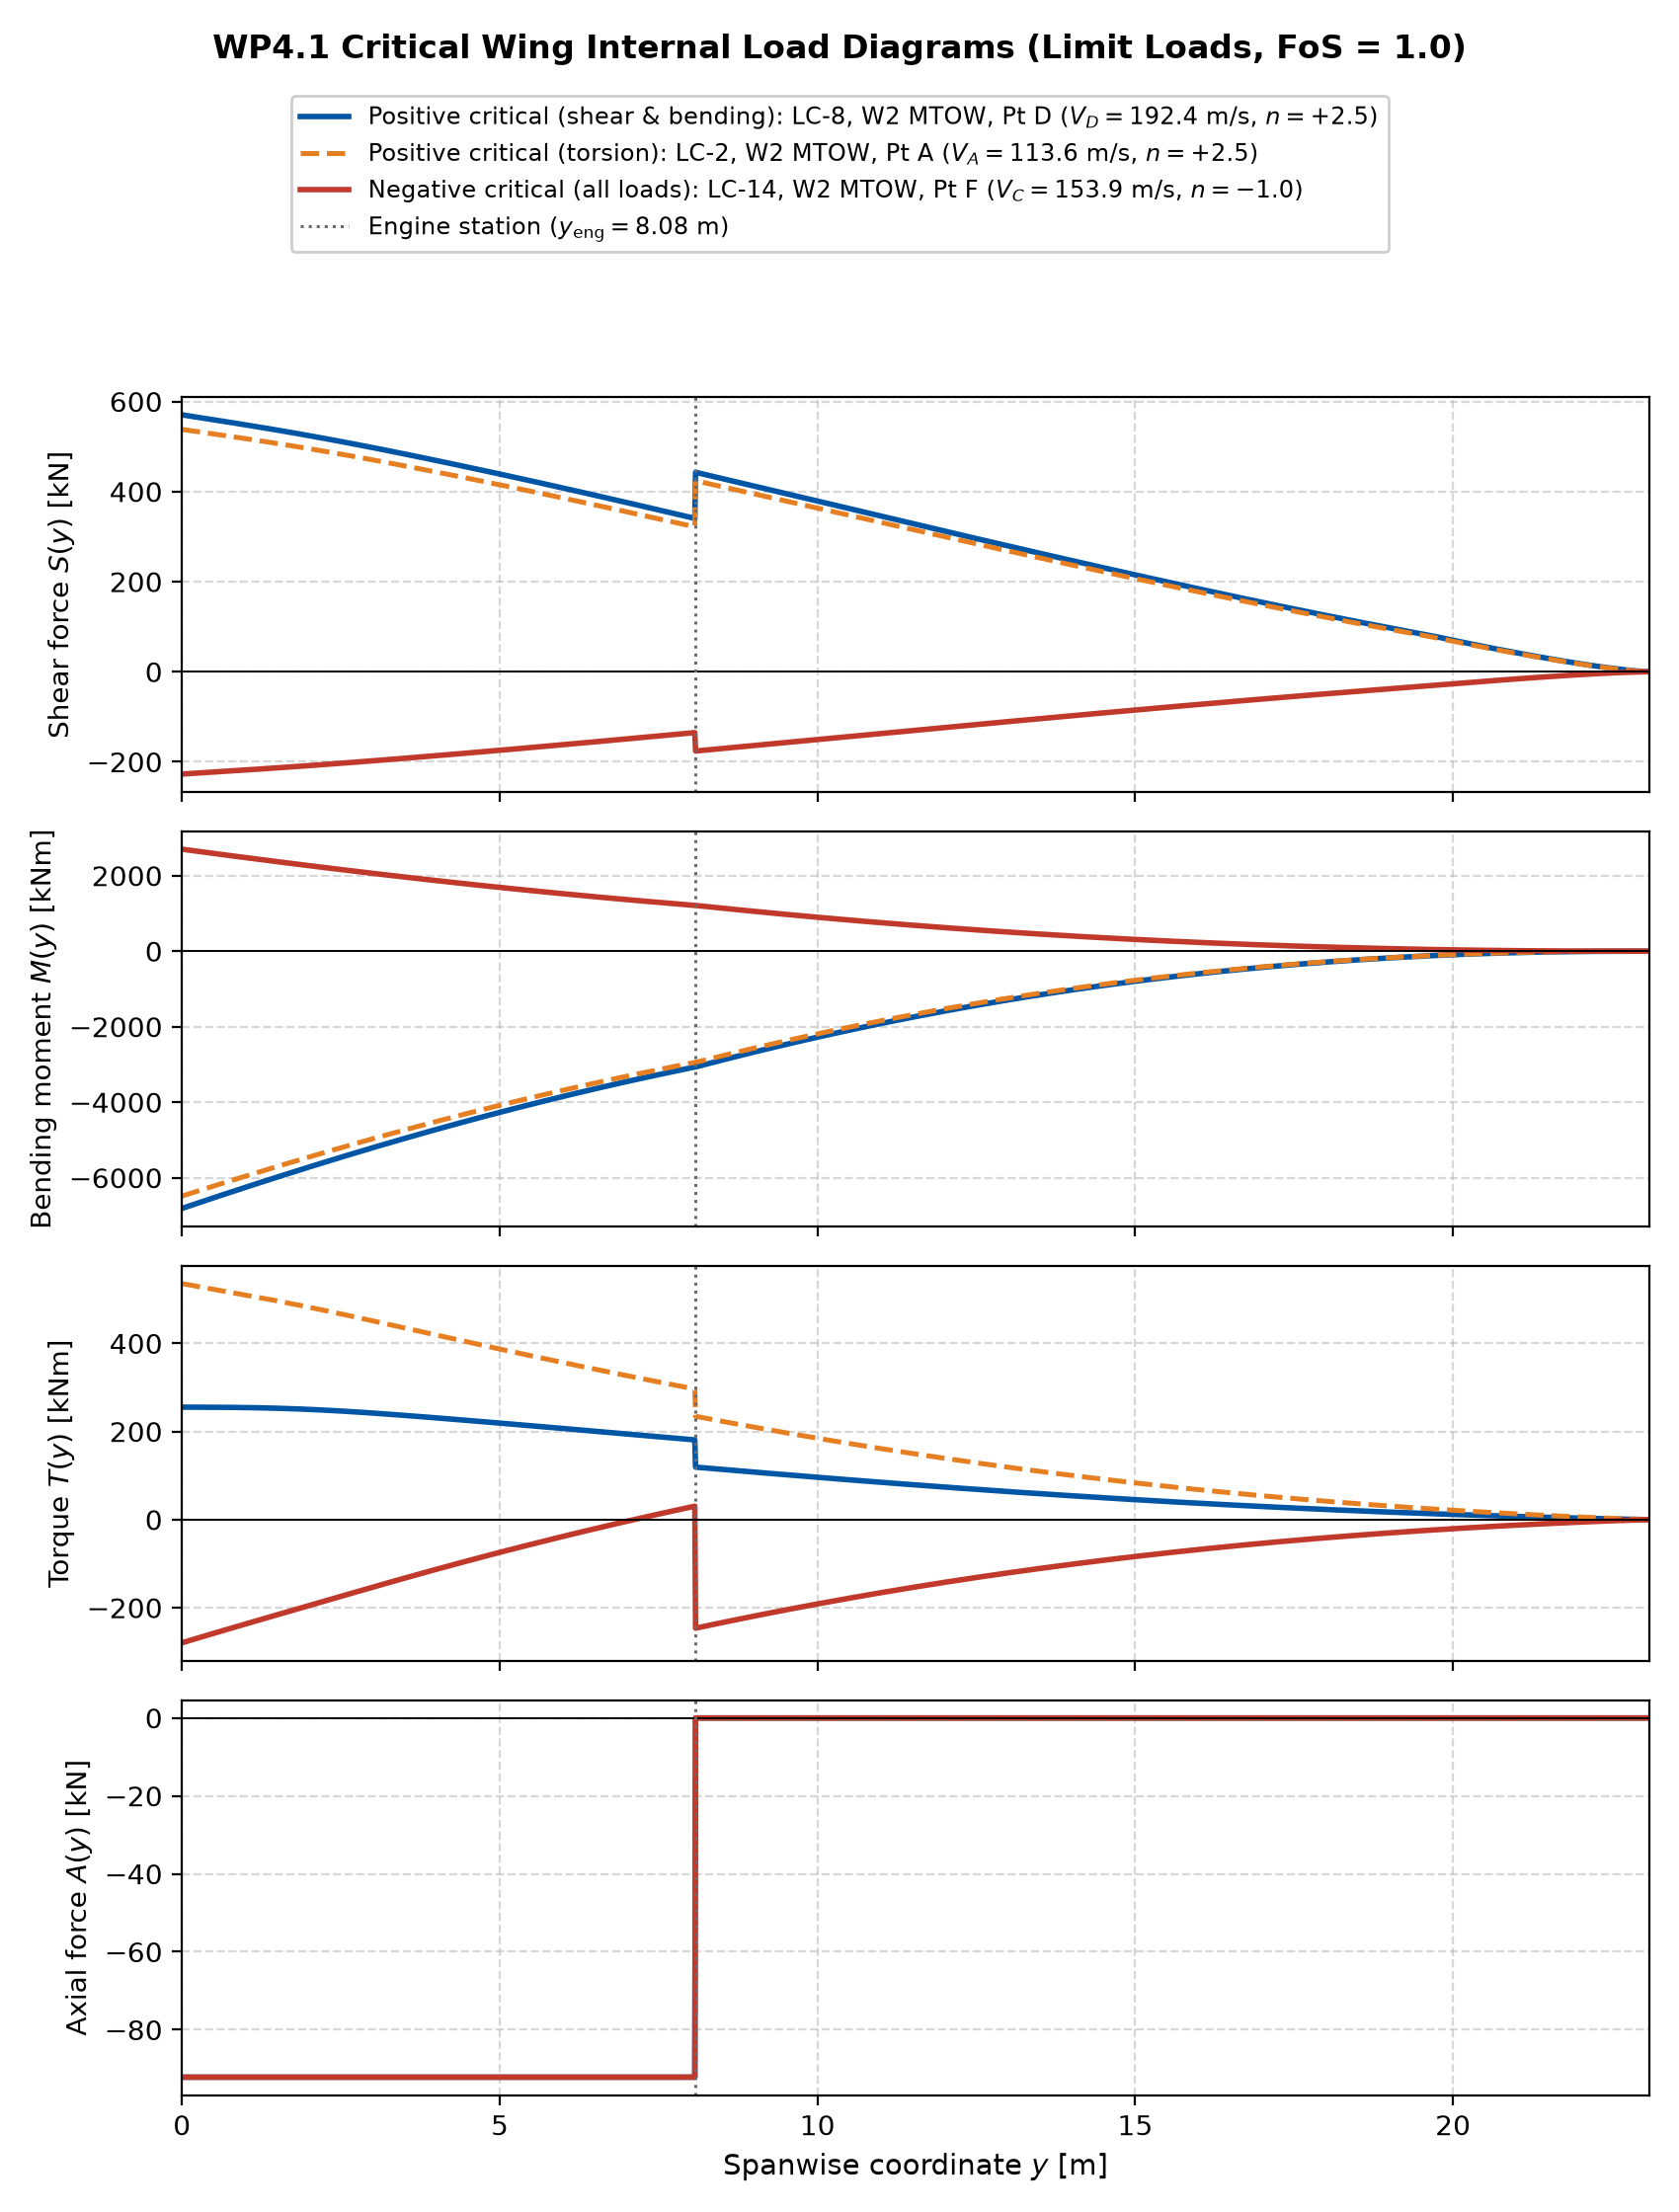
\includegraphics[width=0.95\textwidth]{WP4_1_force_diagrams_combined.png}
    \caption{Spanwise limit internal load diagrams ($S(y)$, $M(y)$, $T(y)$, and $A(y)$) for the critical positive load cases (LC-8 and LC-2, $n = +2.5$) and the critical negative load case (LC-14, $n = -1.0$), all at $W_2$ (MTOW). The vertical dotted line marks the PW2037 engine attachment station ($y_{\mathrm{eng}} = 8.08\,\text{m}$).}
    \label{fig:wp41_combined}
\end{figure}

% Optional: if you prefer individual full-width figures instead of the 4-panel figure above,
% include WP4_1_shear.png, WP4_1_bending_moment.png, WP4_1_torque.png, and WP4_1_axial.png.

\begin{table}[htbp]
    \centering
    \caption{Summary of root limit internal loads ($\mathrm{FoS} = 1.0$) for the selected critical WP4.1 load cases (all at $W_2$: MTOW $= 88{,}515\,\text{kg}$, $m_{\mathrm{fuel}} = 23{,}294\,\text{kg}$).}
    \label{tab:wp41_critical_summary}
    \begin{tabular}{@{}lccccccc@{}}
        \toprule
        \textbf{Load Case} & \textbf{Role} & $n$ & $V_{\mathrm{EAS}}$ & $S(0)$ & $M(0)$ & $T(0)$ & $A(0)$ \\
         & & $[-]$ & $[\text{m/s}]$ & $[\text{kN}]$ & $[\text{kNm}]$ & $[\text{kNm}]$ & $[\text{kN}]$ \\
        \midrule
        LC-8 (Pt~D, SL) & Pos.\ shear \& bending & $+2.5$ & $192.42$ & $+570.4$ & $-6{,}812.4$ & $+255.3$ & $-92.2$ \\
        LC-2 (Pt~A, SL/Cr) & Pos.\ torsion & $+2.5$ & $113.64$ & $+538.0$ & $-6{,}485.4$ & $+535.8$ & $-92.2$ \\
        LC-14 (Pt~F, SL/Cr) & Neg.\ all loads & $-1.0$ & $153.93$ & $-227.2$ & $+2{,}700.5$ & $-279.7$ & $-92.2$ \\
        LC-14 (idle thrust)$^*$ & Neg.\ torsion sensitivity & $-1.0$ & $153.93$ & $-227.2$ & $+2{,}700.5$ & $-495.3$ & $0.0$ \\
        \bottomrule
        \multicolumn{8}{@{}l}{\footnotesize $^*$Sensitivity check with $F_T = 0$: removing the nose-up engine thrust couple increases nose-down root torque.}
    \end{tabular}
\end{table}

Several physical features are visible in Figure~\ref{fig:wp41_combined}. In the shear force diagram, the installed PW2037 engine weight introduces a downward step of $-102.7\,\text{kN}$ at $y_{\mathrm{eng}} = 8.08\,\text{m}$ under $n = +2.5$ (and $+41.1\,\text{kN}$ under $n = -1.0$), producing a distinct slope change in the bending moment curve at the same station. In the torque diagram, the engine introduces a net nose-up couple of $+61.7\,\text{kNm}$ at $n = +2.5$ (where the $+215.7\,\text{kNm}$ thrust couple outweighs the $-154.0\,\text{kNm}$ nose-down weight couple) and $+277.3\,\text{kNm}$ at $n = -1.0$ (where both upward engine inertia and forward thrust act nose-up). Consequently, for LC-14 the torque jumps sharply from $-246.5\,\text{kNm}$ just outboard of the pylon to $+30.5\,\text{kNm}$ just inboard, before the large inboard aerodynamic nose-down moment drives the root torque back to $-279.7\,\text{kNm}$. Finally, the axial force is zero outboard of the engine and constant at $A(y) = -92.2\,\text{kN}$ (compression) inboard of $y_{\mathrm{eng}}$.

% ==============================================================================
\section{Load case justification}
\label{sec:load_case_justification}
% ==============================================================================

The manoeuvre $(V_{\mathrm{EAS}}\text{--}n)$ envelopes derived in Chapter~4 span three weight configurations---$W_1$ (OEW $= 46{,}261\,\text{kg}$), $W_2$ (MTOW $= 88{,}515\,\text{kg}$ with $23{,}294\,\text{kg}$ wing fuel), and $W_3$ (MZFW $= \mathrm{OEW} + \mathrm{MPW} = 65{,}221\,\text{kg}$ with zero fuel)---at two altitudes (sea level and cruise altitude, $h_{\mathrm{cr}} = 9{,}449\,\text{m}$, $\rho = 0.4416\,\text{kg/m}^3$), with CS-25.337 limit load factors $n_{\max} = +2.5$ and $n_{\min} = -1.0$. Before quantitative screening, several subsets of envelope points can be eliminated \textit{a priori}:
\begin{enumerate}
    \item \textbf{Flaps-extended points ($V_F$, $n = +2.0$)}: Excluded directly by Assumption~A17 (control-surface and high-lift deflections are outside the scope of WP4).
    \item \textbf{Operating Empty Weight ($W_1$)}: With $m_{\mathrm{OEW}} = 46{,}261\,\text{kg}$ and zero fuel, $W_1$ generates strictly lower lift and lower net shear and bending moment than $W_2$ and $W_3$ at every load factor and speed.
    \item \textbf{Interior positive boundary points (Point~C at $V_C$, $n = +2.5$)}: Because $V_A < V_C < V_D$ at constant $n = +2.5$, Point~C always produces aerodynamic angles of attack, normal forces, and torques strictly bounded between Point~A and Point~D.
    \item \textbf{Duplicate altitude cases}: Under Assumption~A16 (neglecting Mach effects on $C_{L,\max}$), $V_{S1,\mathrm{EAS}}$, $V_{A,\mathrm{EAS}}$, and $V_{C,\mathrm{EAS}}$ are independent of altitude; hence Points~A, C, F, and H yield identical dynamic pressure $q$ at sea level and cruise. Only the design dive speed $V_D$ depends on altitude: at cruise ($M_C = 0.85$), compressibility limits $M_D = M_C + 0.05 = 0.90$ ($V_{D,\mathrm{EAS}} = 162.99\,\text{m/s}$), whereas at sea level ($M_C = 0.452$) the CS-25.335(b) margin $V_C \le 0.8 V_D$ governs, yielding $V_{D,\mathrm{EAS}} = 192.42\,\text{m/s}$.
\end{enumerate}

To verify these arguments quantitatively and resolve the trade-off between fuel-loaded ($W_2$) and zero-fuel ($W_3$) configurations, all clean-wing envelope corners were evaluated using the numerical model of Section~\ref{sec:derivation_numerical_results}. Table~\ref{tab:wp41_screening} summarises the resulting root internal loads for every unique corner condition.

\begin{table}[htbp]
    \centering
    \caption{Quantitative screening of all unique clean-wing WP4.3 manoeuvre corner load cases (limit loads, $\mathrm{FoS} = 1.0$, $x_{\mathrm{sc}} = 0.40c$). Bold rows denote the selected critical cases.}
    \label{tab:wp41_screening}
    \begin{tabular}{@{}llcccccccc@{}}
        \toprule
        \textbf{Case ID} & \textbf{Config.\ \& Corner} & $n$ & $V_{\mathrm{EAS}}$ & $C_{L,d}$ & $\alpha_d$ & $S(0)$ & $M(0)$ & $T(0)$ \\
         & & $[-]$ & $[\text{m/s}]$ & $[-]$ & $[\text{deg}]$ & $[\text{kN}]$ & $[\text{kNm}]$ & $[\text{kNm}]$ \\
        \midrule
        LC-1 / 4  & $W_1$ (OEW), Pt~A (SL/Cr)     & $+2.5$ & $82.15$  & $+1.545$ & $+17.15$ & $+322.2$ & $-3{,}503.9$ & $+309.5$ \\
        \textbf{LC-2 / 5}  & \textbf{$W_2$ (MTOW), Pt~A (SL/Cr)}    & $\mathbf{+2.5}$ & $\mathbf{113.64}$ & $\mathbf{+1.545}$ & $\mathbf{+17.15}$ & $\mathbf{+538.0}$ & $\mathbf{-6{,}485.4}$ & $\mathbf{+535.8}$ \\
        LC-3 / 6  & $W_3$ (MZFW), Pt~A (SL/Cr)    & $+2.5$ & $97.54$  & $+1.545$ & $+17.15$ & $+547.2$ & $-5{,}759.7$ & $+411.0$ \\
        LC-19 / 22 & $W_1$ (OEW), Pt~C (SL/Cr)    & $+2.5$ & $153.93$ & $+0.440$ & $+3.54$  & $+339.7$ & $-3{,}682.3$ & $+109.1$ \\
        LC-20 / 23 & $W_2$ (MTOW), Pt~C (SL/Cr)   & $+2.5$ & $153.93$ & $+0.842$ & $+8.49$  & $+564.6$ & $-6{,}750.6$ & $+417.9$ \\
        LC-21 / 24 & $W_3$ (MZFW), Pt~C (SL/Cr)   & $+2.5$ & $153.93$ & $+0.620$ & $+5.76$  & $+570.1$ & $-5{,}990.5$ & $+248.5$ \\
        LC-10     & $W_1$ (OEW), Pt~D (Cruise)    & $+2.5$ & $162.99$ & $+0.393$ & $+2.96$  & $+340.0$ & $-3{,}685.5$ & $+73.5$  \\
        LC-11     & $W_2$ (MTOW), Pt~D (Cruise)   & $+2.5$ & $162.99$ & $+0.751$ & $+7.37$  & $+566.7$ & $-6{,}772.2$ & $+383.4$ \\
        LC-12     & $W_3$ (MZFW), Pt~D (Cruise)   & $+2.5$ & $162.99$ & $+0.553$ & $+4.94$  & $+570.9$ & $-5{,}998.9$ & $+213.2$ \\
        LC-7      & $W_1$ (OEW), Pt~D (Sea level) & $+2.5$ & $192.42$ & $+0.282$ & $+1.59$  & $+340.3$ & $-3{,}692.7$ & $-56.7$  \\
        \textbf{LC-8}      & \textbf{$W_2$ (MTOW), Pt~D (Sea level)} & $\mathbf{+2.5}$ & $\mathbf{192.42}$ & $\mathbf{+0.539}$ & $\mathbf{+4.76}$  & $\mathbf{+570.4}$ & $\mathbf{-6{,}812.4}$ & $\mathbf{+255.3}$ \\
        LC-9      & $W_3$ (MZFW), Pt~D (Sea level) & $+2.5$ & $192.42$ & $+0.397$ & $+3.01$  & $+572.2$ & $-6{,}015.3$ & $+83.6$  \\
        \midrule
        LC-25 / 28 & $W_1$ (OEW), Pt~H (SL/Cr)    & $-1.0$ & $51.96$  & $-1.545$ & $-20.91$ & $-124.6$ & $+1{,}357.1$ & $+113.5$ \\
        LC-26 / 29 & $W_2$ (MTOW), Pt~H (SL/Cr)   & $-1.0$ & $71.87$  & $-1.545$ & $-20.91$ & $-207.1$ & $+2{,}509.2$ & $-36.1$  \\
        LC-27 / 30 & $W_3$ (MZFW), Pt~H (SL/Cr)   & $-1.0$ & $61.69$  & $-1.545$ & $-20.91$ & $-212.9$ & $+2{,}241.3$ & $+46.4$  \\
        LC-13 / 16 & $W_1$ (OEW), Pt~F (SL/Cr)    & $-1.0$ & $153.93$ & $-0.176$ & $-4.05$  & $-135.7$ & $+1{,}458.4$ & $-155.2$ \\
        \textbf{LC-14 / 17} & \textbf{$W_2$ (MTOW), Pt~F (SL/Cr)}   & $\mathbf{-1.0}$ & $\mathbf{153.93}$ & $\mathbf{-0.337}$ & $\mathbf{-6.03}$  & $\mathbf{-227.2}$ & $\mathbf{+2{,}700.5}$ & $\mathbf{-279.7}$ \\
        LC-15 / 18 & $W_3$ (MZFW), Pt~F (SL/Cr)   & $-1.0$ & $153.93$ & $-0.248$ & $-4.93$  & $-228.1$ & $+2{,}384.5$ & $-211.1$ \\
        \bottomrule
    \end{tabular}
\end{table}

\subsection{Effect of wing fuel: why $W_2$ (MTOW) governs over $W_3$ (MZFW)}

A classic structural question in wing design is whether maximum zero-fuel weight ($W_3$) is more critical than maximum take-off weight ($W_2$) due to the loss of fuel inertial bending relief. Here, $W_2$ and $W_3$ share the exact same non-fuel fuselage and payload mass ($m_{\mathrm{MTOW}} - m_{\mathrm{fuel},W_2} = m_{\mathrm{MZFW}} = 65{,}221\,\text{kg}$), so adding $23{,}294\,\text{kg}$ of wing fuel leaves the net root vertical shear force virtually unchanged (within $0.32\%$, differing only slightly through $\cos\alpha_d$: $570.4\,\text{kN}$ in LC-8 vs.\ $572.2\,\text{kN}$ in LC-9).

For the bending moment and outboard shear force, however, \textbf{$W_2$ (MTOW) is significantly more critical than $W_3$}. Because of the $32.66^\circ$ sweep, the aerodynamic centre of pressure lies relatively far outboard at $y_{\mathrm{cp}} = 10.03\,\text{m}$ ($43.4\%$ of $b/2$). In contrast, the strong planform taper ($c_t/c_r = 0.292$) concentrates the $c(y)^2$-distributed fuel tank volume near the wing root, placing the fuel centre of gravity at $y_f = 7.16\,\text{m}$ ($31.0\%$ of $b/2$). Consequently, the added fuel increases the aerodynamic bending moment faster than its own inertia relieves it, producing a net bending-moment increase of
\begin{equation}
    \Delta |M(0)| \approx |n|\,g\,\frac{m_{\mathrm{fuel},W_2}}{2}\,(y_{\mathrm{cp}} - y_f)
    = 2.5 \times 9.80665 \times 11{,}647 \times (10.03 - 7.16) \approx 819\,\text{kNm},
    \label{eq:fuel_moment_delta}
\end{equation}
matching the $+797.1\,\text{kNm}$ ($+13.3\%$) increase from LC-9 ($-6{,}015.3\,\text{kNm}$) to LC-8 ($-6{,}812.4\,\text{kNm}$). Outboard of the root, the shear force in $W_2$ also exceeds $W_3$ by $13\text{--}18\%$ (e.g., $442.8\,\text{kN}$ vs.\ $391.3\,\text{kN}$ just outboard of the engine, and $327.3\,\text{kN}$ vs.\ $276.3\,\text{kN}$ at mid-span) because the outer wing carries the higher MTOW lift with very little local fuel mass to oppose it. The same physics holds under $n = -1.0$, where $W_2$ (LC-14) exceeds $W_3$ (LC-15) in bending moment by $+13.3\%$ ($+2{,}700.5\,\text{kNm}$ vs.\ $+2{,}384.5\,\text{kNm}$).

\subsection{Selection of critical positive and negative load cases}

\paragraph{Critical positive load cases ($n = +2.5$):}
Comparing Points~A, C, and D at $W_2$ (MTOW) in Table~\ref{tab:wp41_screening} reveals two distinct physical regimes:
\begin{itemize}
    \item \textbf{LC-8 ($W_2$ MTOW, Point~D at sea level, $V_D = 192.42\,\text{m/s}$, $n = +2.5$)} is the \textbf{primary critical positive load case for shear force and bending moment} ($S(0) = +570.4\,\text{kN}$, $M(0) = -6{,}812.4\,\text{kNm}$). Because sea-level $V_D$ gives the highest dynamic pressure on the envelope, the required $C_{L,d} = 0.539$ is achieved at a small angle of attack ($\alpha_d = 4.76^\circ$, $\cos\alpha_d = 0.997$), maximising the chord-normal aerodynamic load $N'(y)$ relative to Point~A ($\alpha_d = 17.15^\circ$, $\cos\alpha_d = 0.956$). Because bending moment governs the wing-tip vertical deflection requirement (\texttt{REQ-WING-STR-01}) and primary skin/stringer sizing, LC-8 is the governing positive bending case.
    \item \textbf{LC-2 / LC-5 ($W_2$ MTOW, Point~A, $V_A = 113.64\,\text{m/s}$, $n = +2.5$)} is the \textbf{critical positive load case for torsion} ($T(0) = +535.8\,\text{kNm}$, more than double LC-8's $+255.3\,\text{kNm}$). Because the aerodynamic centre ($0.25c$) lies ahead of the shear centre ($0.40c$), upward normal force creates a nose-up moment $N'(0.15c) \approx +650\,\text{kNm}$ that is nearly invariant with speed at constant $nW$, whereas the cambered airfoil pitching moment $m'_{c/4} = q c^2 C_{m,c/4} < 0$ acts nose-down and scales with $V_{\mathrm{EAS}}^2$ ($-175.3\,\text{kNm}$ at $V_A$ vs.\ $-475.6\,\text{kNm}$ at sea-level $V_D$). At minimum manoeuvring speed $V_A$, this opposing nose-down pitching moment is smallest, maximising positive (nose-up) torque and therefore governing positive wing-tip twist (\texttt{REQ-WING-STR-02}) in Chapter~3.
\end{itemize}

\paragraph{Critical negative load case ($n = -1.0$):}
\textbf{LC-14 / LC-17 ($W_2$ MTOW, Point~F, $V_C = 153.93\,\text{m/s}$, $n = -1.0$)} is unambiguously the single most critical negative load case across all internal loads ($S(0) = -227.2\,\text{kN}$, $M(0) = +2{,}700.5\,\text{kNm}$, $T(0) = -279.7\,\text{kNm}$). Compared to Point~H ($V_{S1} = 71.87\,\text{m/s}$, $\alpha_d = -20.91^\circ$), the higher dynamic pressure at $V_C$ reduces $|\alpha_d|$ to $6.03^\circ$, increasing $|N'(y)|$ and root bending moment by $+7.6\%$. Simultaneously, in negative-$g$ flight the downward aerodynamic normal force acting ahead of the shear centre ($-267.5\,\text{kNm}$) and the high-$q$ cambered-airfoil pitching moment ($-289.5\,\text{kNm}$) both act \textbf{nose-down}, making Point~F the worst-case negative torsion condition by a wide margin. Moreover, as shown in Table~\ref{tab:wp41_critical_summary}, if the engines are throttled to idle during a negative-$g$ pushover ($F_T = 0$), the counteracting nose-up thrust couple vanishes and the root nose-down torque increases to $-495.3\,\text{kNm}$; this idle-thrust condition should therefore be checked when verifying negative twist and spar-web shear buckling in Chapter~3 and WP5.
